\section{Shape systematics in the non-resonant results}
\label{sec:shapesyst}

The BSM search for non-resonant HH is done based in the benchmarks defined by the cluster analysis. 
The bechmark classification is based in kinematic properties of the signal. The method 
provides a map between the portion of the parameter space reasonably described by the 
topology of each one of the benchmarks defined by the parameters displayed in Tab.~\ref{tab:bench}. 

To allow the interpretation of the experimental limit derived in the benchmarks 
in the whole parameter space with the mapping of~\cite{Dall'Osso:2015aia} we follow 
the prescription on~\cite{CarvalhoAntunesDeOliveira:2130724}, that we brieflly 
describe bellow:

In figure~\ref{fig:out_mass} we show an example of the comparison between the benchmark (in black), 
with the other samples that belong to the same cluster (in light brown and other collors), to cluster 3.
A subset of samples that envelope the all the other samples of the cluster, so called outliers, is defines in three mass points  $m_{\rm HH\,,1}\,\equiv$ 270\,GeV, $m_{\rm HH\,,2}\,\equiv$ 400\,GeV and $m_{\rm HH\,,3}\,\equiv$ 600\,GeV, applied to a histogram with 20\,GeV wide bins. The first and last mass points are intended to catch
the analysis sensitivity to threshold region ($\mHH \approx 2 m_{\PH}$) and energy-tail modifications. The
intermediate mass point is close to the typical valley found
in the distribution due to a cancellation between the different diagrams, and it is intended
to catch the analyses sensitivity to short-distance fluctuations in shape. 
One may observe that the choice of outliers in $\mHH$ is also reasonably valid for other distributions, like the 
H boson $p_T$~\cite{CarvalhoAntunesDeOliveira:2130724}. 
As result, six outliers are defined. The same procedure is done to the 12 clusters, the result in terms of model parameters 
is found in the mentioned reference. 

Using the reweighting procedure described in Sec.~\ref{sec:rewei} we are able to produce limits for the 
outliers. {\bf 	RESULTS, LETS HOPE FOR NO SUBCLUSTERING}

\begin{figure*}[h]\begin{center}
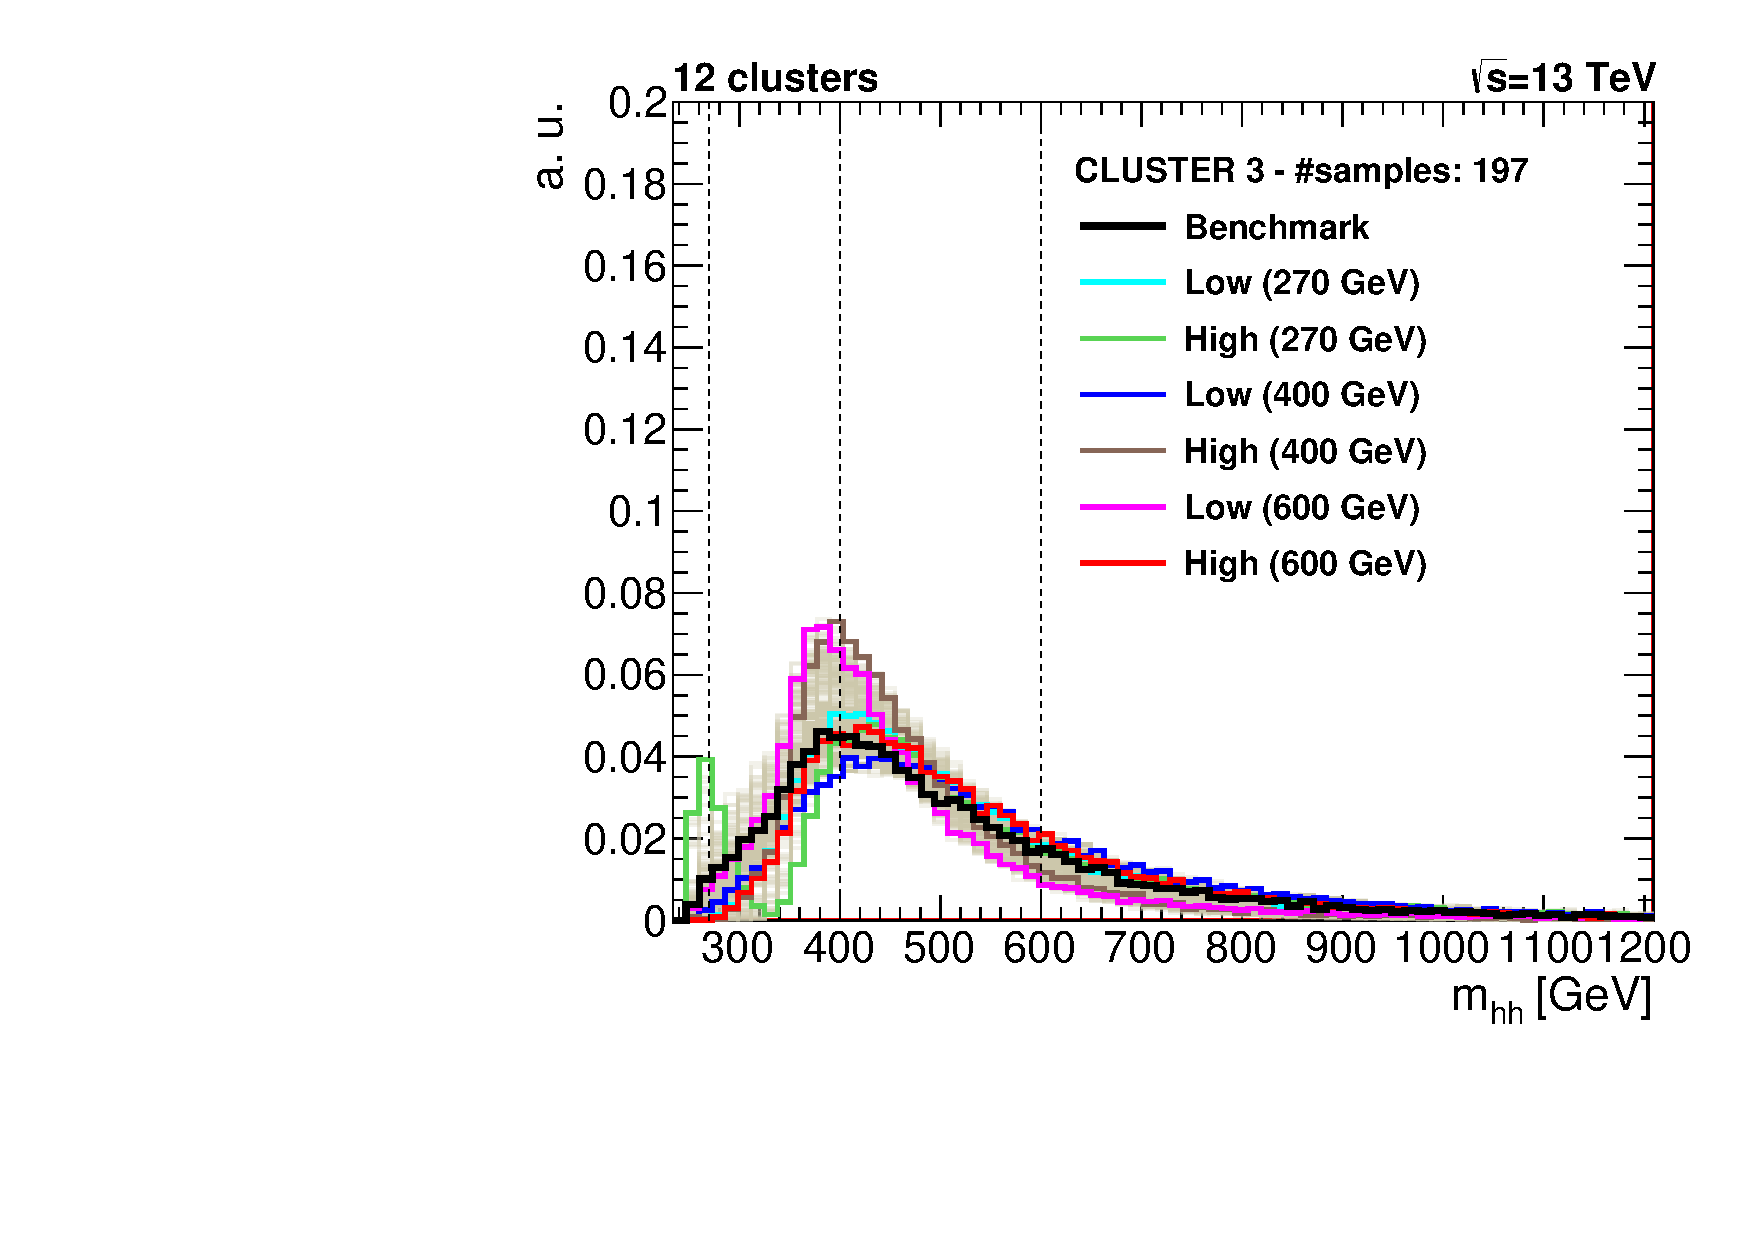
\includegraphics[width=0.41\textwidth, angle =0 ]{figures/envelope/5par_13Tev_Nclu12_Clus3_mhh.pdf}
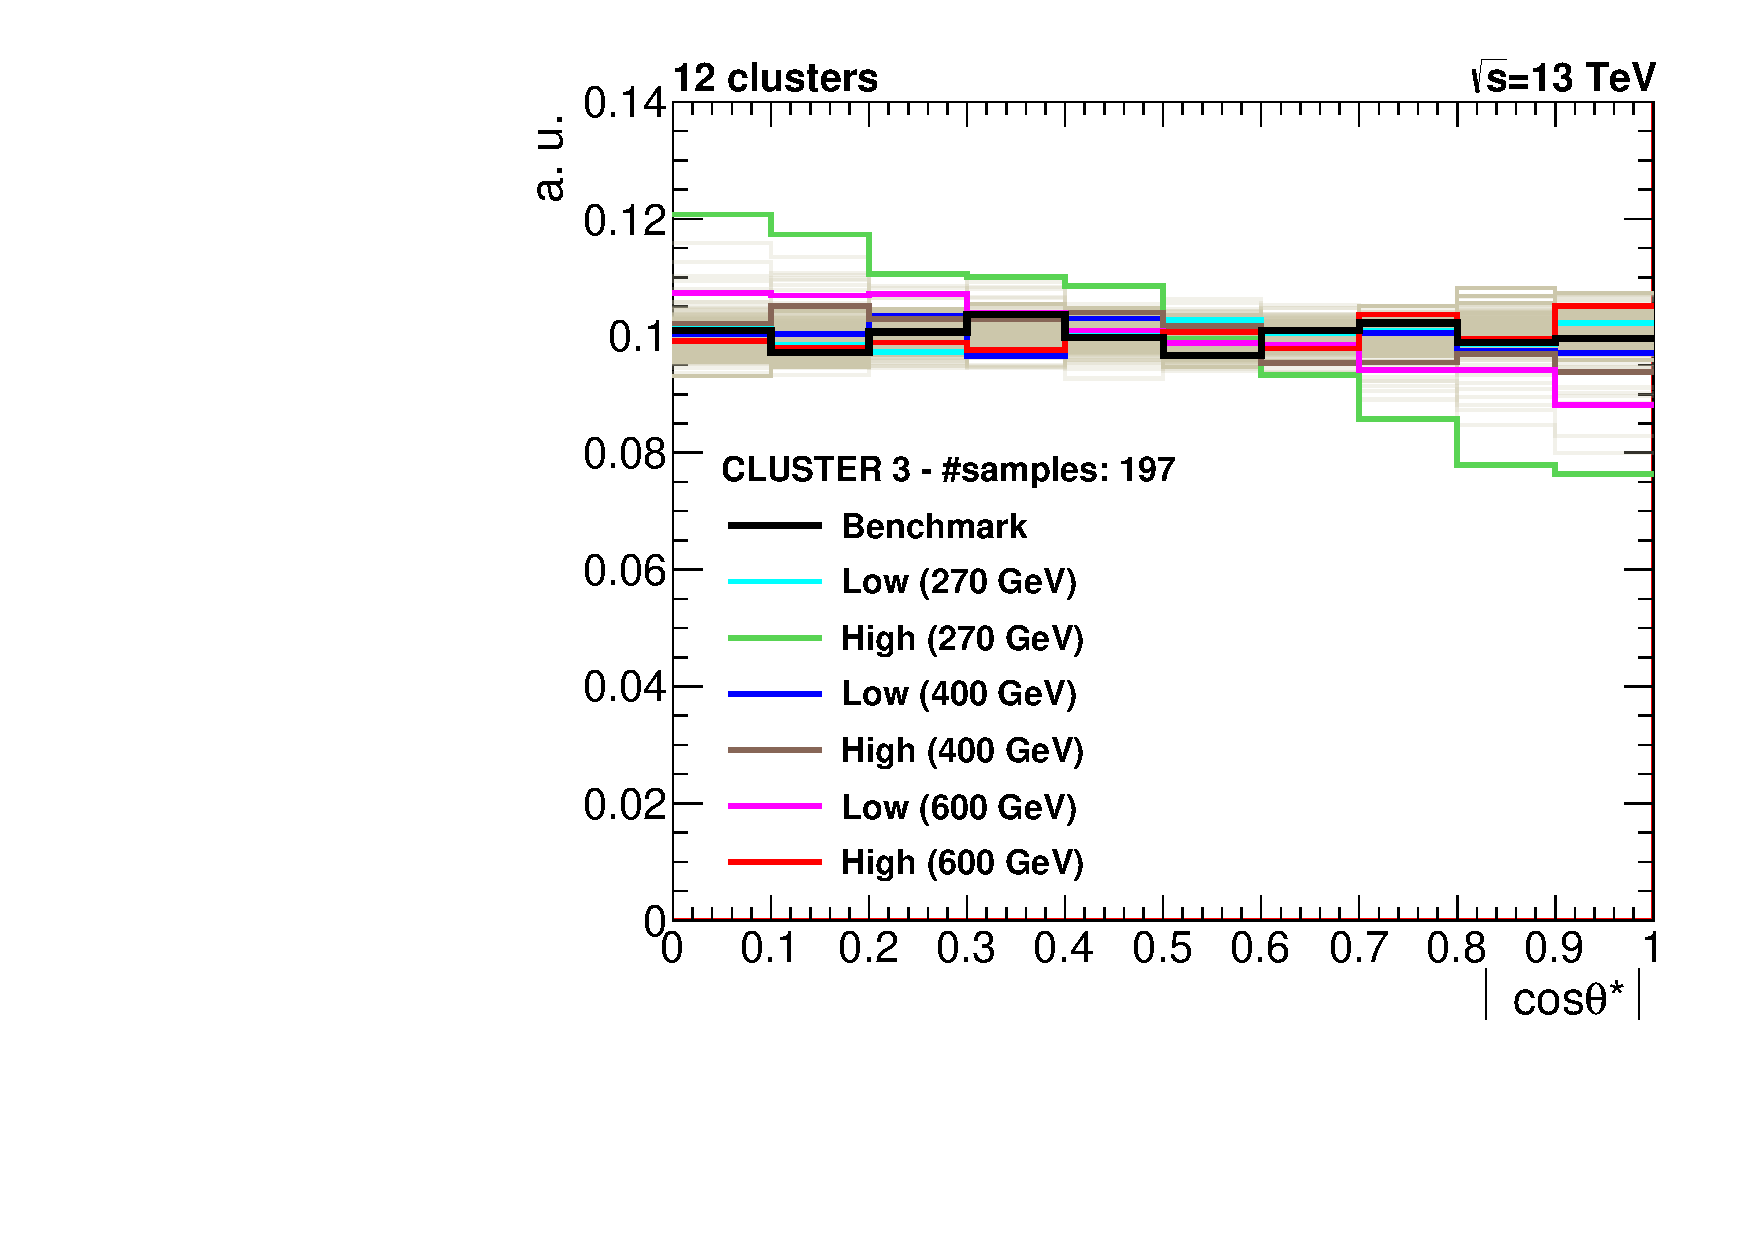
\includegraphics[width=0.41\textwidth, angle =0 ]{figures/envelope/5par_13Tev_Nclu12_Clus3_hcths.pdf}
%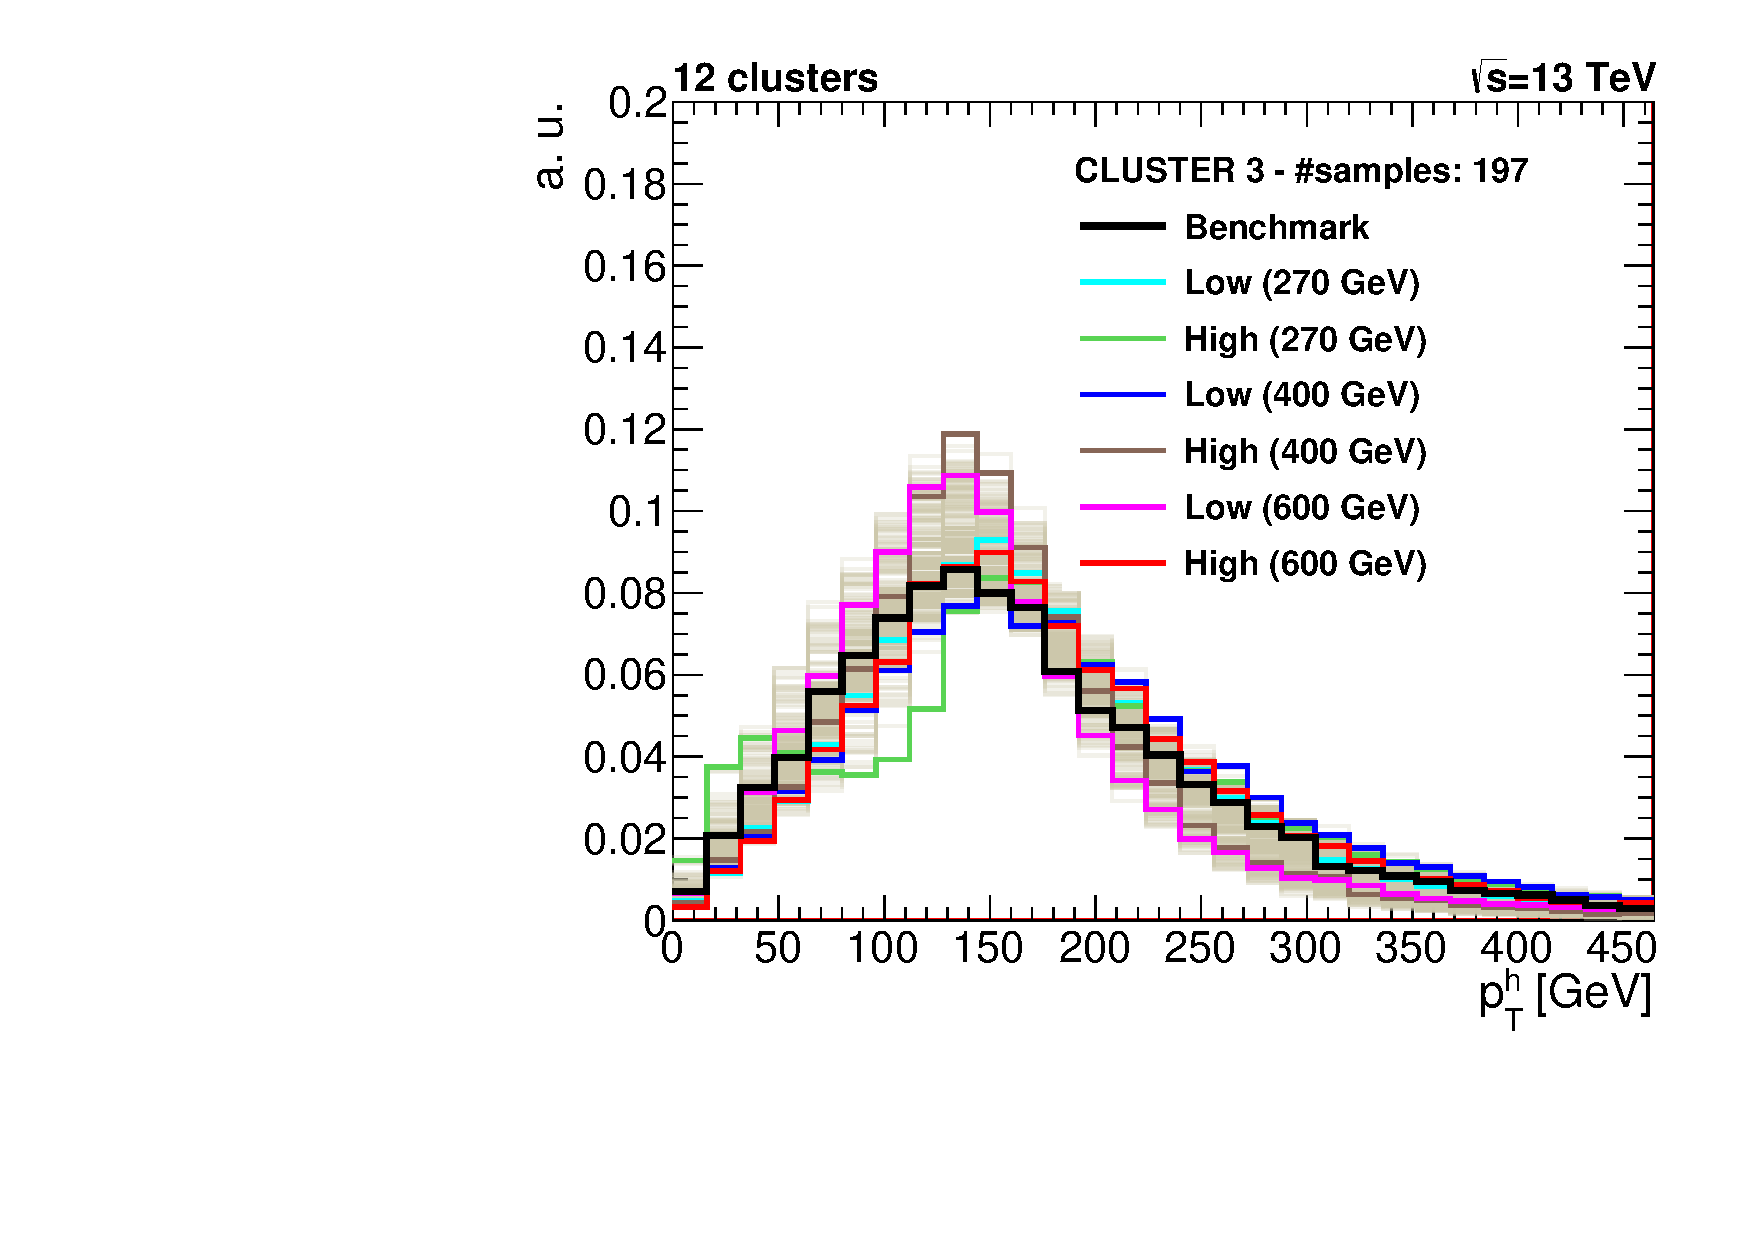
\includegraphics[width=0.41\textwidth, angle =0 ]{figures/envelope/5par_13Tev_Nclu12_Clus3_pt.pdf}
\caption{\small  The $\mHH$ ( left) and $|\cos \theta^{*}|$ (right) distributions for the members of cluster 3. The benchmark (in black color) and corresponding outliers (colored lines) are highlighted. The three mass regions are indicated by vertical dashed lines. Figure taken from~\cite{CarvalhoAntunesDeOliveira:2130724}. 
{\bf MAKE THE RECO AS COMPARISON}
\label{fig:out_mass}}
\end{center}\end{figure*}




